\documentclass[border=6pt]{standalone}
\usepackage{tikz}
\usetikzlibrary{arrows.meta,positioning,fit,calc,backgrounds}
\definecolor{fg}{HTML}{DBC9A8}
\definecolor{fgbody}{HTML}{C4A882}
\definecolor{stroke}{HTML}{C4963C}
\definecolor{surf}{HTML}{22222B}
\definecolor{surfemph}{HTML}{2A2820}
\definecolor{surfact}{HTML}{2E2020}
\definecolor{bdim}{HTML}{9A7F62}
\definecolor{bemph}{HTML}{D4A849}
\definecolor{bact}{HTML}{FF5C5C}
\begin{document}
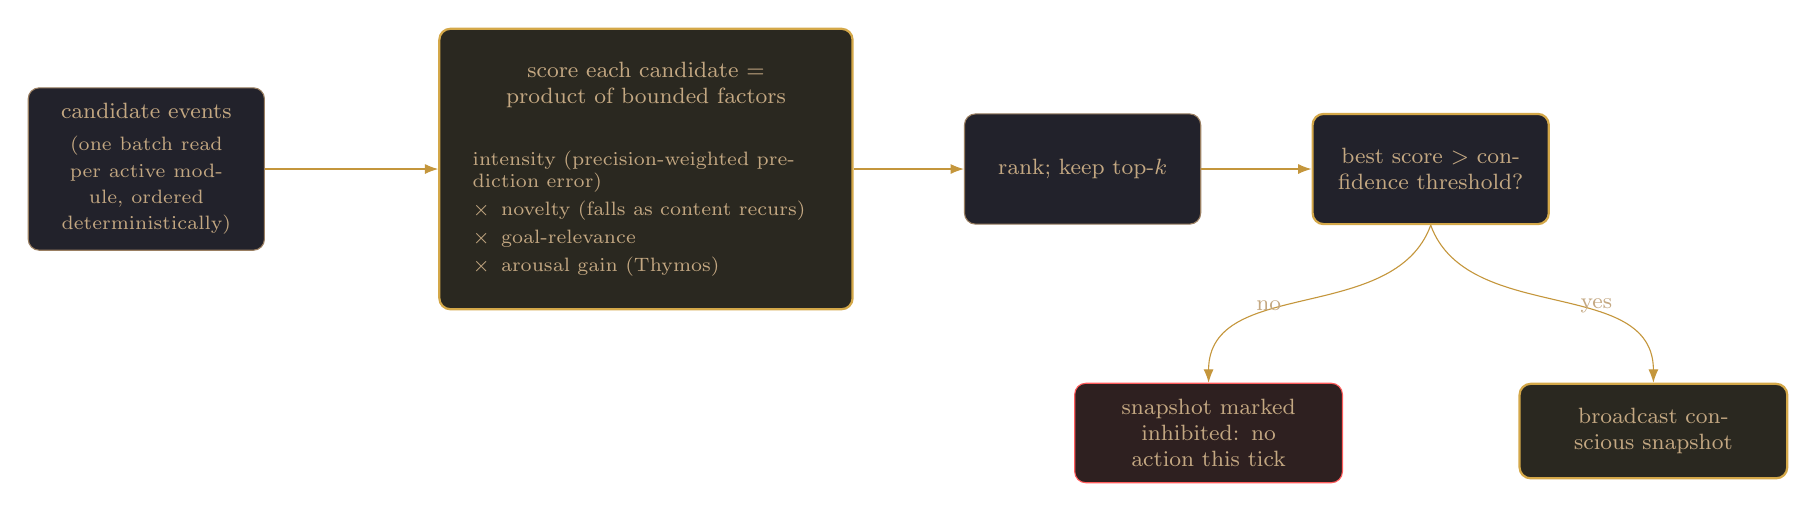
\begin{tikzpicture}[
  font=\small,>=Latex,
  every node/.append style={text=fgbody},
  stage/.style={draw=bdim, rounded corners, fill=surf, align=center, minimum height=14mm, font=\footnotesize, text width=26mm, inner sep=2mm},
  decide/.style={draw=bemph, thick, rounded corners, fill=surf, align=center, minimum height=14mm, font=\footnotesize, text width=26mm, inner sep=2mm},
  sel/.style={draw=bemph, thick, rounded corners, fill=surfemph, align=center, minimum height=12mm, font=\footnotesize, text width=30mm, inner sep=2mm},
  halt/.style={draw=bact, rounded corners, fill=surfact, align=center, minimum height=12mm, font=\footnotesize, text width=30mm, inner sep=2mm},
]
% (b) the scoring box, at the origin, factor list inside it
\node[align=center, font=\footnotesize, text width=44mm] (scoretitle) at (0,0)
  {score each candidate $=$ product of bounded factors};
\node[align=left, font=\scriptsize, text width=44mm, below=3mm of scoretitle] (scorelist)
  {intensity (precision-weighted prediction error)\\[2pt]
   $\times$\, novelty (falls as content recurs)\\[2pt]
   $\times$\, goal-relevance\\[2pt]
   $\times$\, arousal gain (Thymos)};
\begin{pgfonlayer}{background}
\node[draw=bemph, thick, rounded corners, fill=surfemph, fit=(scoretitle)(scorelist), inner sep=3mm] (score) {};
\end{pgfonlayer}
% (a) candidate events
\node[stage, left=22mm of score] (cand) {candidate events\\[2pt]\scriptsize (one batch read per active module, ordered deterministically)};
% (c) rank
\node[stage, right=14mm of score] (rank) {rank; keep top-$k$};
% (d) decision
\node[decide, right=14mm of rank] (dec) {best score $>$ confidence threshold?};
% branches
\node[sel,  below right=20mm and -4mm of dec] (yes) {broadcast conscious snapshot};
\node[halt, below left=20mm and -4mm of dec] (no) {snapshot marked inhibited: no action this tick};
% arrows
\draw[->, draw=stroke] (cand) -- (score);
\draw[->, draw=stroke] (score) -- (rank);
\draw[->, draw=stroke] (rank) -- (dec);
\draw[->, draw=stroke] (dec.south) to[out=250,in=90] node[left, font=\footnotesize, pos=0.55]{no} (no.north);
\draw[->, draw=stroke] (dec.south) to[out=290,in=90] node[right, font=\footnotesize, pos=0.55]{yes} (yes.north);
\end{tikzpicture}
\end{document}
